\styledchapter[Hoe werkt Machine Learning?]{hoe-werkt-machine-learning}

\Gls{machine-learning} is onderdeel van het domein \gls{computer-science}. Binnen \gls{machine-learning} worden algoritmische modellen gebouwd om statistische problemen op te lossen. Dit wordt gedaan met behulp van een dataset dat verzameld is uit de echt wereld of gefabriceerd door mensen. Het model kan met behulp van de dataset een redelijk nauwkeurige voorspelling maken \cite[p.~7]{the-hundred-page-machine-learning-book}.

Hoe het niet AI is -> https://machinelearningmastery.com/think-machine-learning/

\section{Hoe leert een machine learning model?}\label{sec:hoe-leert-een-machine-learning-model}
Een \gls{machine-learning} model leert met behulp van een dataset om een voorspelling te maken. Een dataset kan duizenden \glspl{machine-learning-feature-vector} (voorbeelden) bevatten, waarbij elke vector een of meerdere \glspl{machine-learning-feature} (attribuut) heeft. In een voorbeeld waarbij een model moet kunnen voorspellen of een persoon kanker heeft kan een \gls{machine-learning-feature-vector} één persoon zijn en de \glspl{machine-learning-feature} het gewicht, leeftijd, lengte en of de persoon kanker heeft \cite{google-ml-terminology}.

Het model gaat langs alle \glspl{machine-learning-feature-vector} en probeert correlaties te vinden tussen de features. Op basis hiervan kan het model vervolgens een voorspelling doet met een \gls{machine-learning-feature-vector} dat het model nooit heeft gezien.

Er zijn een aantal manieren om een algoritme te laten trainen, gegroepeerd in vier vormen.

\subsection{Supervised learning}\label{subsec:supervised-learning}
Met \gls{supervised-learning} wordt een model getraind door middel van een \textbf{gelabeld} dataset. Dit betekent dat een \gls{machine-learning-feature-vector} gepaard gaat met de gewenste label.

\begin{table}[hbt!]
  \centering
  \begin{tabular}{|l|l|}
  \hline
  \textbf{Feature} & \textbf{Label} \\ \hline
  woorden, afzender, tijd van versturen&spam/geen spam\\ \hline
  \end{tabular}
  \caption{Voorbeeld gelabeld dataset}
  \label{table:voorbeeld-gelabeld-dataset}
\end{table}

Het model kan leren dat woorden zoals 'gratis' in e-mails die tussen 01:00 en 03:00 worden verstuurd vaak als spam gelabeld zijn. Het model kan concluderen dat als een e-mail met dezelfde features als input word gegeven, dat het een spam e-mail is \cite{google-ml-terminology}.

\subsection{Unsupervised learning}\label{subsec:unsupervised-learning}
\Gls{unsupervised-learning} lijkt grotendeels op \gls{supervised-learning}. Het verschil is dat de \glspl{machine-learning-feature-vector} in de dataset niet gepaard zijn met een label. 

\begin{table}[hbt!]
  \centering
  \begin{tabular}{|l|l|}
  \hline
  \textbf{Feature} & \textbf{Label} \\ \hline
  woorden, afzender, tijd van versturen&?\\ \hline
  \end{tabular}
  \caption{Voorbeeld niet gelabeld dataset}
  \label{table:voorbeeld-niet-gelabeld-dataset}
\end{table}

Het doel bij \gls{unsupervised-learning} is om de data op een bepaalde manier te transformeren om er iets waardevols uit te halen. Een voorbeeld hiervan is het \textit{clusteren} van data. Hierbij wordt soortgelijke data gegroepeerd (\autoref{fig:clustering-example}). Een andere voorbeeld is \textit{dimensionality reduction} (\autoref{fig:dimensionality-reduction-example}). \Gls{machine-learning-feature} worden weggelaten om twee \glspl{machine-learning-feature} tegen over elkaar te zetten om bijvoorbeeld uitschieters te vinden \cite{the-hundred-page-machine-learning-book}.

\begin{figure}[hbt!]
    \centering
    \begin{minipage}{0.3\textwidth}
        \centering
        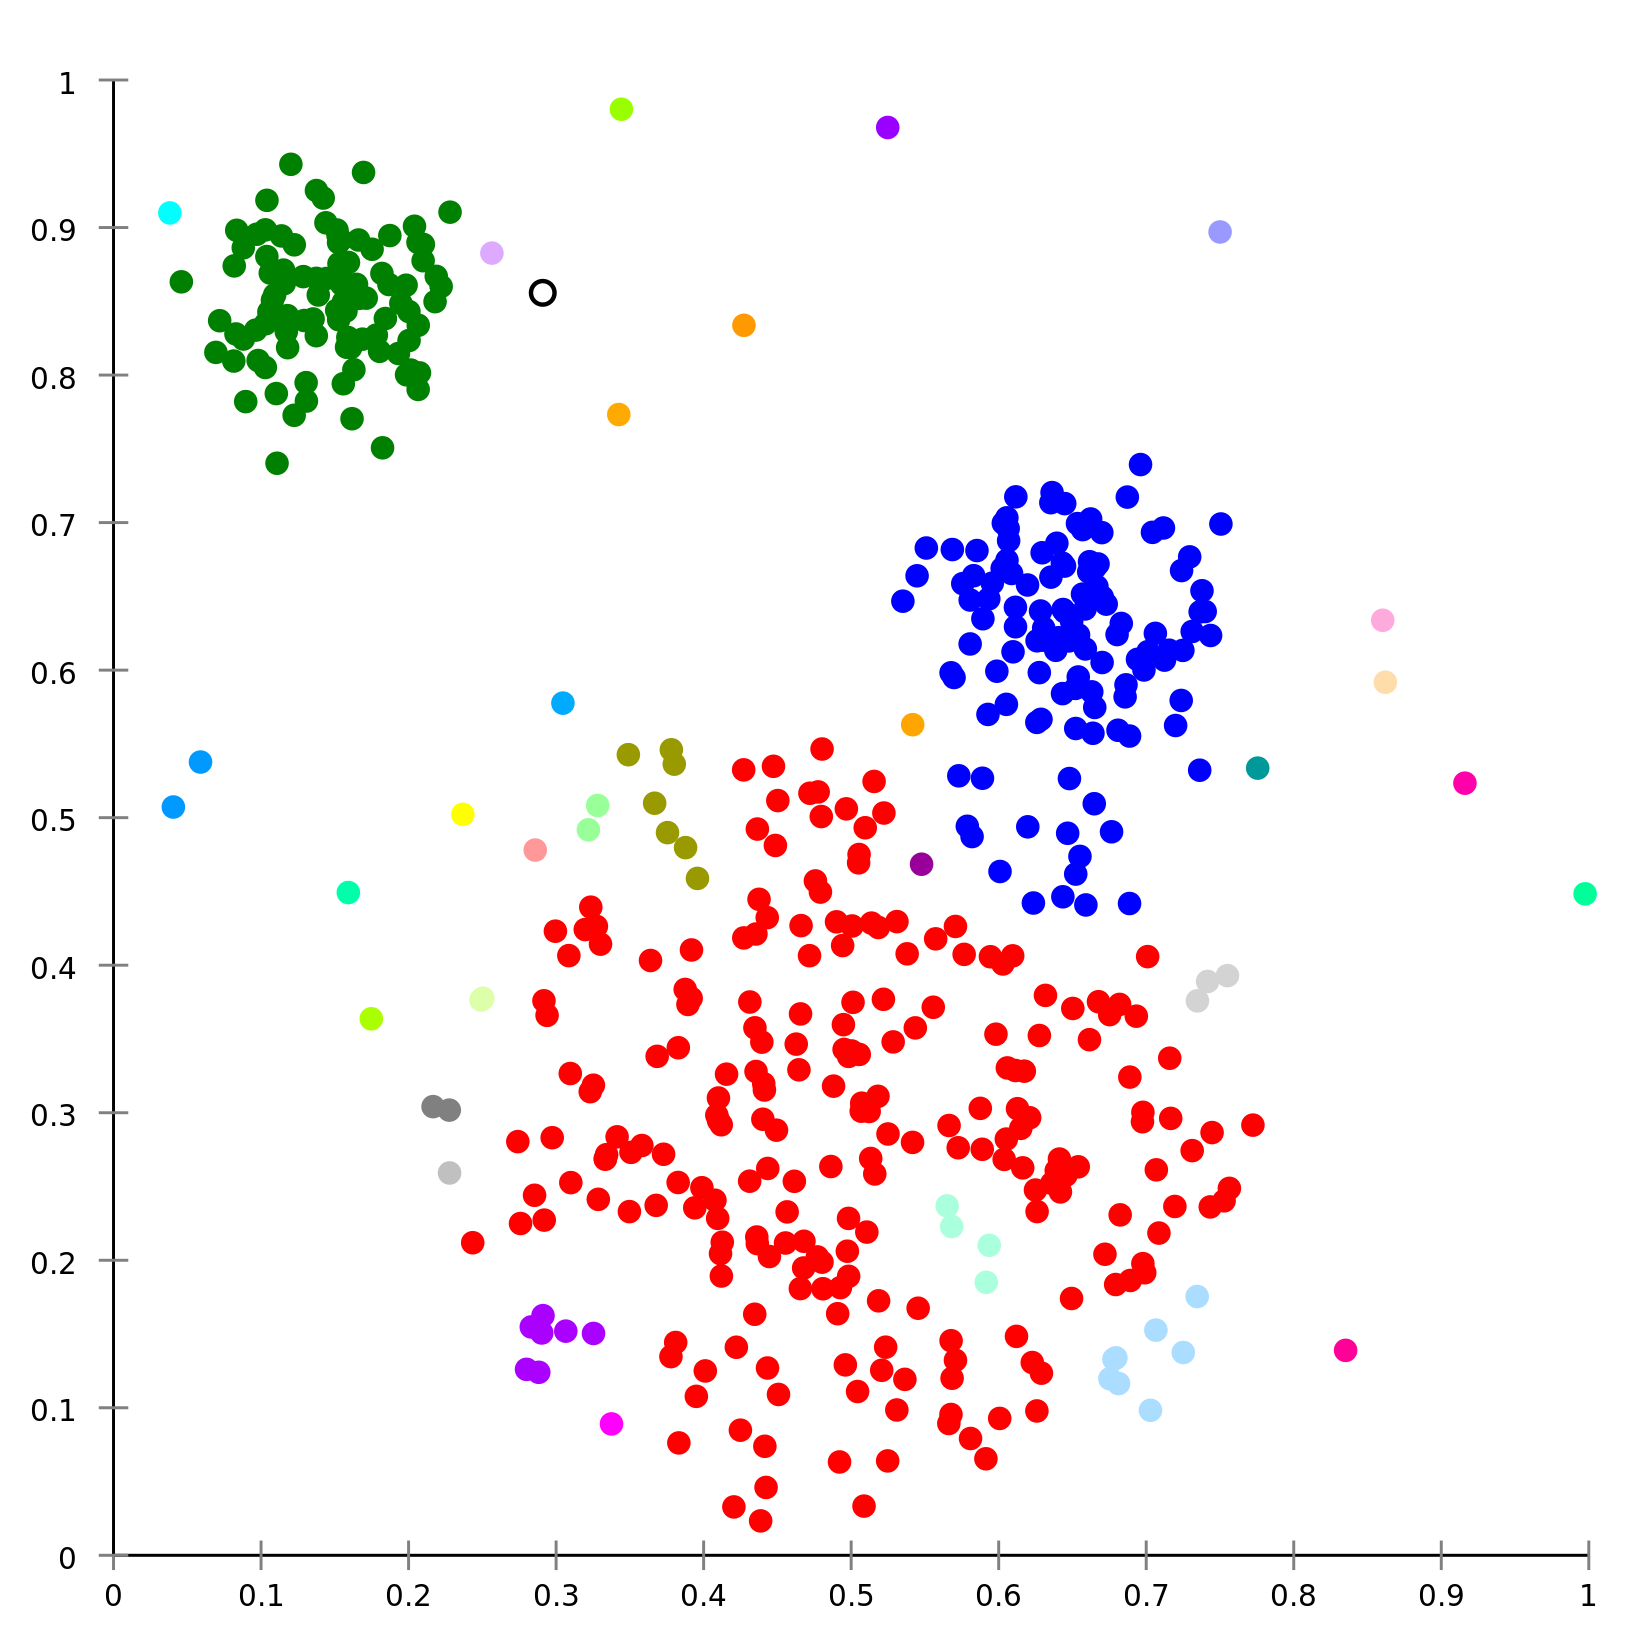
\includegraphics[width=0.9\textwidth]{./chapter-5/clustering-example.png}
        \caption{Voorbeeld van \textit{clustering}}
        \label{fig:clustering-example}
    \end{minipage}\hfill
    \begin{minipage}{0.6\textwidth}
        \centering
        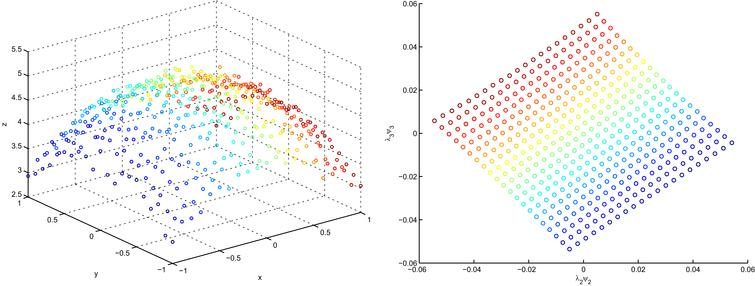
\includegraphics[width=0.9\textwidth]{./chapter-5/dimensionality-reduction-example.jpg}
        \caption{Voorbeeld van \textit{dimensionality reduction}}
        \label{fig:dimensionality-reduction-example}
    \end{minipage}
\end{figure}

\subsection{Semi-supervised learning}\label{subsec:semi-supervised-learning}
\Gls{semi-supervised-learning} is een combinatie van \gls{supervised-learning} en \gls{unsupervised-learning} waarbij het doel dezelfde is als \gls{supervised-learning}. Het is gebruikelijk dat het merendeel van de dataset niet gelabelde data is \cite{the-hundred-page-machine-learning-book}.

\subsection{Reinforcement learning}\label{subsec:reinforcement-learning}
\Gls{reinforcement-learning} wordt ook wel 'survival learning' genoemd. Een analogie hiervoor is een organisme dat moet overleven in verschillende situaties door de juiste actie te verrichten. Acties kunnen een positief of een negatief effect hebben. Acties dat langdurig een positieve effect hebben moeten versterkt worden zodat het model zo veel mogelijk positieve acties verricht \cite{bayesian-reasoning-and-machine-learning-book}.

\section{Stappenplan voor het trainen van een model}\label{sec:stappenplan-voor-het-trainen-van-een-model}
Het trainen van een model neemt een klein gedeelte in beslag van het hele proces. Vooraf moet het probleem worden gedefinieerd waarna vervolgens de data wordt verzameld. Het is belangrijk om de data grondig te verkennen want als het model traint met onbruikbare data, is het model ook onbruikbaar. Dit heet ook wel garbage in = garbage out. Na het verkennen kan de data opgeschoond worden. Dit wordt gedaan met de garbage in = garbage out regel in gedachte; hoe beter de data, hoe beter het model zal presteren. \Gls{feature-engineering} is het tegenovergestelde van het opschonen van de dataset. Waarbij data wordt weggehaald, wordt er nieuwe data geïntroduceerd. Dit wordt gedaan met de bestaande data en zorgt ervoor dat belangrijke elementen van de dataset worden aangestipt voor het model. Voor het trainen van het model moet de dataset gesplitst worden in een training dataset en test dataset. Daarna kan het model getraind worden met behulp van het afstemmen van model- en hyperparameters en \gls{cross-validation}. Model- en hyperparameters zijn 'instellingen'
voor het model en met \gls{cross-validation} kunnen verschillende instellingen worden getest met alleen de training dataset. Als laatste kan een model gekozen worden dat het beste presteert \cite{data-science-primer}.

Deze stappen kunnen verschillen.
Kan voorkomen dat je meer stappen moet doen of andere.
Sommige modellen vereisen specifieke handelingen, deze stappen zijn voor de meest gebruikte.

\subsection{Data verkennen}\label{subsec:data-verkennen}
Bij het verkennen wordt gekeken welke \glspl{machine-learning-feature} kunnen worden gebruikt. Het kan handig zijn om de data te plotten in bijvoorbeeld een histogram, een staafdiagram of een boxplot. \cite{data-science-primer} Het plotten kan handig zijn voor het vinden van:

\begin{itemize}
  \item uitschieters
  \item meetfouten
  \item features die gescheiden het model negatief kunnen beïnvloeden, maar samen positief
\end{itemize}

Vervolgens kunnen er correlaties tussen variabelen gevonden worden. Variabelen in een dataset kunnen gerelateerd aan elkaar zijn op een aantal manieren. Brownlee \cite{ml-correlation-brownlee} geeft een aantal voorbeelden:

\begin{itemize}
  \item Een variabele kan de waarde van een andere variabele veroorzaken of hiervan afhankelijk zijn
  \item Een variabele kan lichtelijk geassocieerd zijn met een ander variabele
  \item Twee variabele kan afhankelijk zijn van een derde onbekende variabele
\end{itemize}

Een correlatie kan positief wat betekent dat de variabelen in dezelfde richting bewegen, bijvoorbeeld het gewicht en de lengte van een persoon. Het kan ook negatief zijn. Dit betekent dat als één variabele de ene kant op gaat, de andere variabele de tegengestelde richting op gaat. Een voorbeeld hiervan is het aantal tentamens en recreative tijd. Bij een neutrale correlatie betekent het dat de variabelen niks met elkaar te maken hebben \cite{ml-correlation-brownlee}.

De relatie tussen twee variabelen heet de \gls{covariantie}. Met een formule kan de \gls{covariantie} worden berekent:

\[cov(X, Y) = (sum (x - mean(X)) * (y - mean(Y)) ) * 1/(n-1)\]

Waarbij het resultaat het volgende kan zijn:

\[[[385.33297729, 389.7545618] [389.7545618, 500.38006058]]\]

Omdat dit moeilijk te interpreteren kan zijn, werden er coëfficiënten bedacht. Twee daarvan zijn de \textit{Pearson correlation coefficient} en de \textit{Spearman correlation coefficient}. De achterliggende formule verschillen, maar het resultaat moet de \gls{covariantie} in context brengen. Het resultaat uit een coëfficiënt formule is een getal tussen de \(1\) en \(-1\), waarbij \(1\) een positieve correlatie is en een \(-1\) een negatieve correlatie. Er is geen correlatie als het resultaat een \(0\) is. Vaak is er een correlatie als er een waarde boven \(0,5\) en onder \(-0,5\) voorkomt.

\subsection{Data opschonen}\label{subsec:data-opschonen}
Voor het opschonen van data is er geen beste manier omdat elk dataset verschilt van elkaar. Toch kunnen een aantal vuistregels aangehouden worden om na deze stap een betere dataset te hebben. Als eerst kan er gekeken worden welke data weg kan. Dit kan duplicaten zijn of data dat niet relevant is. Na het weggooien moet structurele fouten worden gecorrigeerd als ze voorkomen. Dit zijn fouten zoals typefouten, woorden die de ene keer wel hoofdletter zijn maar de andere keer niet, fout gelabelde data, enz.

Een optionele stap is om uitschieters weg te gooien. Het kan voorkomen dat uitschieters het model negatief beïnvloeden. Als dat het geval is, kan de uitschieter uit de dataset weggehaald worden.  

Als laatste stap is het belangrijk om te kijken of er data mist. Hiervoor zijn er twee manieren op dit te verhelpen: het weglaten van data of infereren. Helaas zijn beide manieren sub-optimaal omdat er bij het weglaten kostbare data wordt weggegooid en het infereren is natuurlijk niet accuraat \cite{data-science-primer}.

\subsection{Feature engineering}\label{subsec:feature-engineering}
Bij \gls{feature-engineering} worden er nieuwe input features gemaakt die bestaan uit bestaande features. Het nut hiervan is dat er informatie aangestipt kan worden voor het model wat relevant is. Een manier hiervan is om 'interactie features' te maken. Hierbij worden twee features samengevoegd tot een derde feature. Een voorbeeld van het maken van een interactie feature:

\begin{quoting}
  Een model moet kunnen voorspellen of een huis op de huizenmarkt het goed gaat doen. De dataset bevat een aantal features waaronder \textit{num\_schools} en \textit{median\_school}. \textit{num\_schools} is het aantal scholen binnen een radius van 5km van het huis en \textit{median\_school} het gemiddelde van alle scholen in de radius.
  
  Er kan beargumenteerd worden dat een huis beter verkoopt als er \textbf{veel scholen in de buurt zijn} die ook \textbf{een hoge score hebben}. Er kan een nieuwe feature gemaakt worden genaamd \textit{school\_score} dat wordt berekent door \textit{num\_schools} \(*\) \textit{median\_school} te doen. \textit{school\_score} is de interactie feature.
\end{quoting}

Een tweede manier om features te maken is om bestaande features samen te voegen. Dit is handig om te doen als de features los van elkaar niet vaak voorkomen in de dataset én samenhang hebben met elkaar. 

\subsection{Een model trainen}\label{subsec:model-trainen}
Voordat het model getraind kan worden, moet de dataset gesplitst worden in een training dataset en een test dataset. Het is gebruikelijk om de dataset te splitsen in 80\% training en 20\% test of 50\% training en 50\% test; hiervoor is er geen vaste regel en hangt af van de dataset en het model. De dataset wordt gesplitst om \gls{overfitting} te voorkomen. Een model dat overfit is presteert met een hoge accuraatheid op de training dataset, maar laag op een dataset dat het model nog nooit heeft gezien. Door een test dataset apart te houden kan er gevalideerd worden of het model goed presteert met data dat het model nog nooit heeft gezien \cite{data-science-primer}.

Tijdens het trainen en voorspellen werkt het model met \glspl{model-parameter} en \glspl{model-hyperparameter}. \Glspl{model-parameter} zijn interne variabelen van het model die niet expliciet gespecificeerd zijn. \Glspl{model-hyperparameter} worden daarin tegen wel handmatig gespecificeerd en kan bijvoorbeeld het aantal leersessies zijn \cite{ml-model-hyper-parameter-brownlee}. Het vinden van de juiste waarde van \glspl{model-hyperparameter} kan alleen met experimenteren worden achterhaald \cite{data-science-primer}.

Omdat de test dataset niet kan worden gebruikt tijdens het experimenteren moet er gebruik worden gemaakt van \gls{cross-validation}. Er zijn een aantal manieren om \gls{cross-validation} uit te voeren waarbij \textbf{10-fold cross-validation} een van de meest gebruikte is. Bij deze methode wordt de training dataset opgesplitst in 10 delen, ook wel \glspl{fold} genoemd, waarvan 1 een \textit{holdout} \gls{fold} is. Het model zal met de 9 \glspl{fold} trainen en wordt getest met de holdout \gls{fold}. Dit zal 10 keer gedaan worden met elke keer een andere holdout fold zoals weergegeven in \autoref{fig:10-k-cross-validation}. Na elke train sessie wordt een score berekent dat wordt opgeteld bij de andere sessies. Hiervan wordt het gemiddelde berekend en het resultaat is de \textit{cross-validated score}. Hoe hoger dit resultaat, hoe beter het model presteert \cite{data-science-primer}.

\begin{figure}[hbt!]
  \centering
  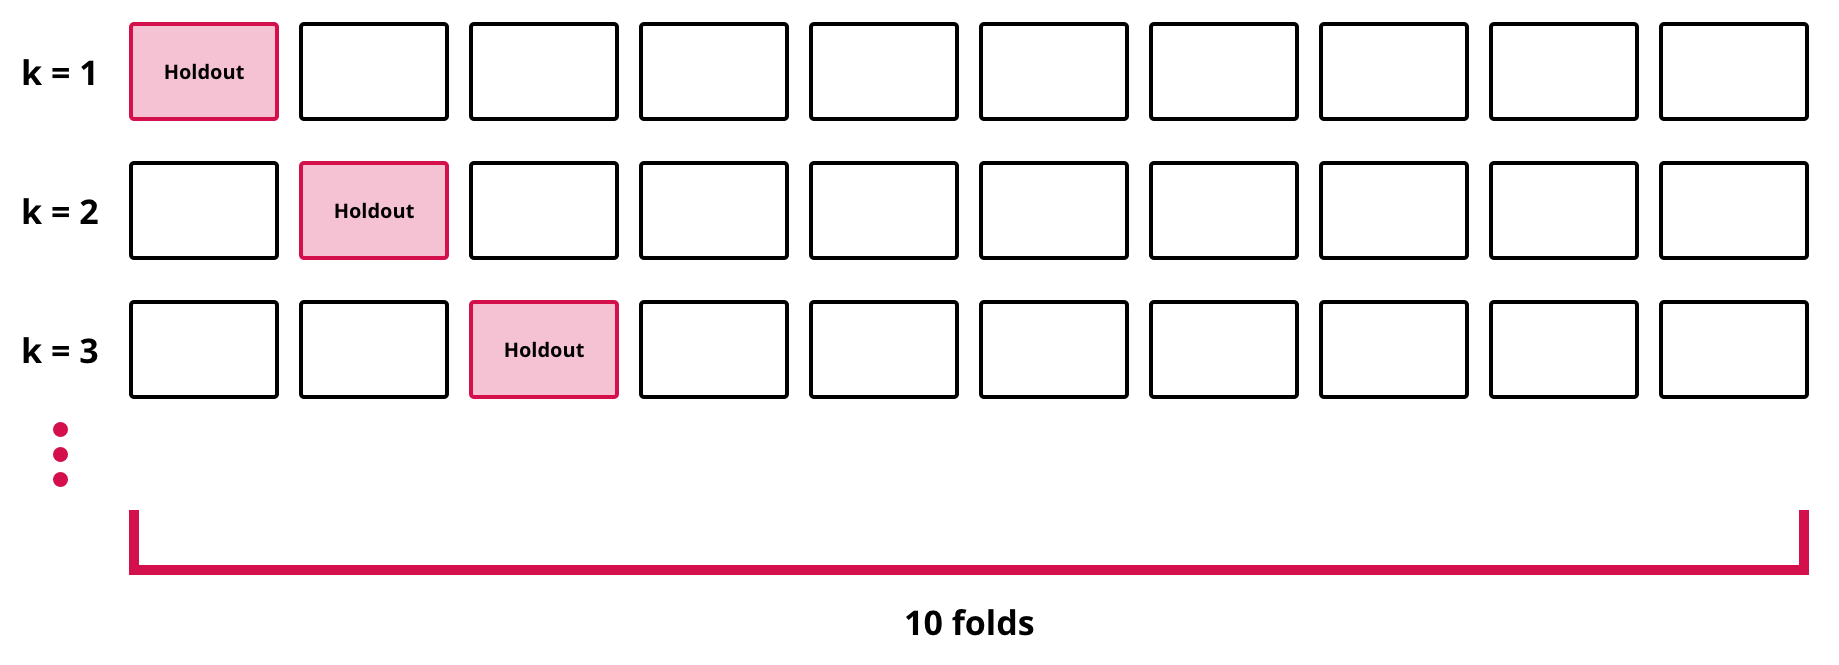
\includegraphics[width=15cm]{./chapter-5/10-k-cross-validation.png}
  \caption{Visualisatie van de 10-k cross-validation methode}
  \label{fig:10-k-cross-validation}
\end{figure}

Om de beste set van parameters te achterhalen kan 10-k cross-validation  toegepast worden op elke set. De cross-validated scores kunnen met elkaar worden vergeleken om de beste \gls{model-hyperparameter} voor het model te achterhalen. Een voorbeeld van de tests op een set is te zien in \autoref{fig:10-k-cross-validation-on-each-model-hyperparameter-set}.

\begin{figure}[hbt!]
  \centering
  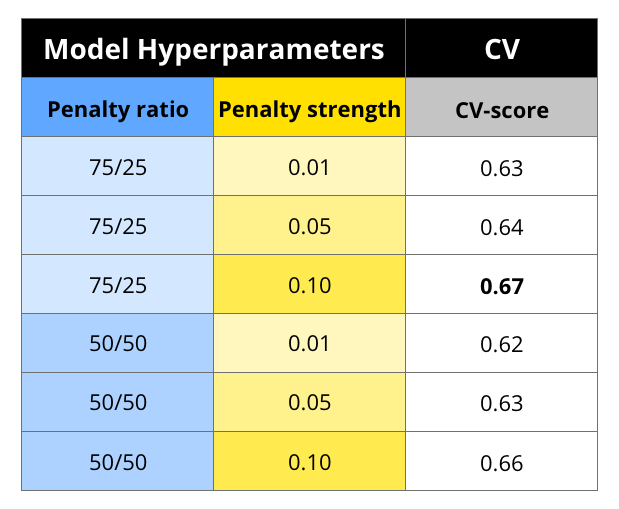
\includegraphics[width=9cm]{./chapter-5/10-k-cross-validation-on-each-model-hyperparameter-set.png}
  \caption{Test matrix op elke model hyperparameter set}
  \label{fig:10-k-cross-validation-on-each-model-hyperparameter-set}
\end{figure}

\bigskip\bigskip\bigskip\bigskip\bigskip\bigskip\bigskip\bigskip
Nu de 'beste' model hyperparameters zijn gevonden, kan het model getest worden tegen de test dataset. Er zijn een aantal prestatiestatistieken waarmee gekeken kan worden hoe goed het model presteert. Voor regressie modellen is \textbf{Mean Squared Error (MSE)} of \textbf{Mean Absolute Error (MAE)} aanbevolen waarbij het model beter presteert als het getal lager is \cite{data-science-primer}. Voor classificatie modellen is de \textbf{Area Under ROC Curve (AUROC)} aanbevolen waar het model juist beter presteert als het getal hoger is \cite{data-science-primer}.

\section{Kennis vereist om een model te trainen}\label{sec:kennis-vereist-om-een-model-te-trainen}


\section{Wachttijden voorspellen}\label{sec:wachttijden-voorspellen}


\section{Conclusie}\label{sec:conclusie}


\section{Advies}\label{sec:advies}
